\section{Method}
\label{sec:method}

\autoref{fig:pipeline} provides an overview of our method. Details of the pipeline are described in the following subsections.

\begin{figure*}[t]
    \centering
    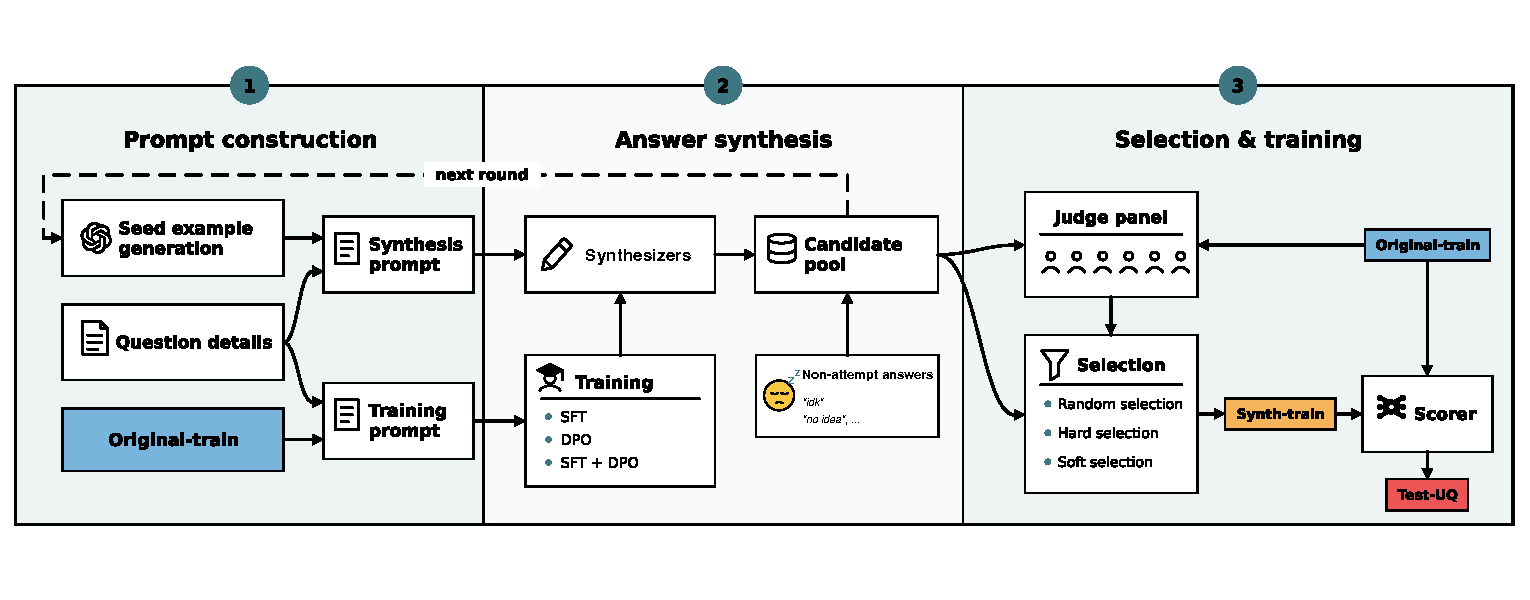
\includegraphics[width=\textwidth]{figures/fig1_pipeline.pdf}
    \caption{Overview of the training and evaluation pipeline.}
    \label{fig:pipeline}
\end{figure*}

\subsection{Dataset}
\label{sec:dataset}

% We use the three-way versions of BEETLE and SciEntsBank~\citep{dzikovskaSemEval2013Task2013}, with answers labeled incorrect, partially correct, or correct. Each example contains a question, a reference answer, a student answer, and its score level. \autoref{tab:dataset-statistics} summarizes the original training and test splits. UA denotes unseen answers, UQ denotes unseen questions, and UD denotes unseen domains. Our cross-question evaluation focuses on BEETLE UQ and SciEntsBank UQ and UD, whose questions are disjoint from the training questions; their real student answers are reserved for evaluation.

% For each split, we report the number of questions $Q$, the number of student answers $N$, and the mean number of answers per (question, score level) pair, $N/(3Q)$. This mean includes all three score levels for every question, including pairs with no observed answers. Training counts are reported before holding out 10\% of the original training set for validation.
We use the BEETLE and SciEntsBank datasets~\citep{dzikovskaSemEval2013Task2013}, reformulating the original five-way label scheme as a three-level scheme (incorrect, partially correct, correct), as in prior work~\citep{sun-etal-2026-rubric}. The unseen-question (UQ) and unseen-domain (UD) splits of SciEntsBank are used for cross-question evaluation. The latter one is a harder transfer task as it test the model on completely unseen subjects. \autoref{tab:dataset-statistics} in \autoref{app:datasets} summarizes the original training and test splits.

% \paragraph{Training Protocol}
% For the SFT synthesizers, we train for 800 steps. For the DPO synthesizers without SFT, we train for 1200 steps. For the DPO synthesizers with SFT, we train for 800 steps.

\subsection{Prompt Construction}
\label{sec:prompt-construction}

Each prompt is built for a question $q$ and a requested level $\ell$ and asks the model to generate new answers that differ from the seed examples. \autoref{tab:synthesis-prompt} in \autoref{app:synthesis-prompt} shows an example.

\paragraph{Question Context Augmentation.}
To better capture the requirements of each question and the scoring criteria for each level, \textit{gpt-5-mini} augments the question with a context description and a set of rubrics for each level. A detailed example of the question context and rubrics is shown in \autoref{tab:question-metadata} in \autoref{app:question-metadata}.

\paragraph{Seed Examples.}
During training, the seed examples are 10 real student answers from the training set for each question and level. For unseen questions, the seeds, contexts, and rubrics are derived from unlabeled answers pseudo-labeled by the judge panel (\autoref{app:seed-examples}).

\paragraph{Target Examples.}
To train the synthesizers via SFT or DPO, we randomly sample 10 real student answers from the training set for each question and level as the target examples.

\paragraph{Diversity Filter.}
To encourage diversity in the generated answers, we apply a diversity filter during training to the seed examples and the target examples, both \textbf{between} the targets and the seed examples and \textbf{among} the targets themselves. The cosine-similarity threshold between sentence embeddings\footnote{sentence-transformers/paraphrase-multilingual-mpnet-base-v2.} is 0.95, or 1.0 for correct answers, where \textbf{legitimate near-duplicates} are common.



\subsection{Answer Synthesis}
\label{sec:answer-synthesis}

We compare four synthesis approaches. Few-shot prompting uses off-the-shelf models, while the other three use models fine-tuned only on real answers to seen questions.

\paragraph{Few-shot prompting.}
As a baseline, synthesis prompts are sent directly to four instruction-tuned LLMs.\footnote{The full model list is given in \autoref{app:synthesizer-training}.}

\paragraph{Supervised fine-tuning (SFT).}
Each of the three open models is fine-tuned on the training prompts, with the real student answers as the target completions.



\paragraph{Level-contrastive preference tuning (DPO).}
Realistic synthetic answers for ASAS must capture the nuanced differences between adjacent score levels. SFT only raises the likelihood of the real answers at the requested level but never teaches the model to distinguish between adjacent levels, so we use direct preference optimization (DPO)~\citep{rafailovDirectPreferenceOptimization2023} on pairs of real answers (\autoref{fig:dpo-pairs}). For a training prompt $x$ with requested level $\ell$, the chosen completion $y^{+}$ lists real answers at level $\ell$, and the rejected completion $y^{-}$ lists real answers to the same question at an adjacent level $\ell'$, with $|\ell - \ell'| = 1$. The loss has two terms. The DPO term prefers $y^{+}$ over $y^{-}$, which teaches the synthesizer to separate adjacent levels. The NLL term is the SFT loss on $y^{+}$~\citep{pangIterativeReasoningPreference2024}: it maximizes the likelihood of the real answers at the requested level, since the DPO term alone only widens the margin and can lower the likelihood of $y^{+}$ itself.
\begin{gather}
\mathcal{L} = \mathbb{E}\Bigl[-\log \sigma\bigl(h_\theta(y^{+}) - h_\theta(y^{-})\bigr) + \alpha\,\mathcal{L}_{\mathrm{NLL}}(y^{+})\Bigr], \label{eq:dpo} \\
h_\theta(y) = \beta \log \frac{\pi_\theta(y \mid x)}{\pi_{\mathrm{ref}}(y \mid x)}. \notag
\end{gather}
Here $\pi_\theta$ is the synthesizer, $\pi_{\mathrm{ref}}$ is a frozen reference model, $\beta$ and $\alpha$ are hyperparameters (\autoref{app:synthesizer-training}), and $\mathcal{L}_{\mathrm{NLL}}$ is the per-token negative log-likelihood of $y^{+}$. Negative examples are filtered so that their answer lengths match those of the positive examples\footnote{We allow a difference of up to 10\% of the mean length.}, which prevents DPO from using 
\textit{length as a shortcut}, since answers tend to be longer at higher levels.

\begin{figure}[t]
    \centering
    \definecolor{dpochosen}{HTML}{2457A6}
    \definecolor{dporejected}{HTML}{B4472E}
    \begin{tikzpicture}[
        every node/.style={font=\scriptsize},
        prompt/.style={draw=black, fill=black!4, inner sep=3pt, outer sep=0pt, text width=0.96\columnwidth, align=left, anchor=north},
        level/.style={inner sep=3pt, text width=0.285\columnwidth, minimum height=1.95cm, align=flush center, anchor=north},
        chosen/.style={level, draw=black, thick, fill=dpochosen!10},
        rejected/.style={level, draw=black, dashed, fill=dporejected!6},
    ]
        \node[prompt, label={[anchor=south west, inner sep=1pt]north west:Prompt $x$}] (level) at (0,0) {\textbf{Requested level: partially correct}};
        \node[prompt] (x) at (level.south) {%
            \textbf{Question:} Explain why you got a voltage reading of 1.5 for terminal 1 and the positive terminal.\\
            \textbf{Context:} The question asks why a voltmeter read 1.5 V between terminal 1 and the positive terminal. \dots\\
            \textbf{Rubric:} States at least one of the necessary components correctly but omits others. \dots};
        \path (x.south) ++(0,-0.3) coordinate (row);
        \node[rejected] (incorrect) at ([xshift=-0.335\columnwidth]row) {\strut\textcolor{dporejected}{rejected $y^{-}$}\\[1pt]\textbf{Incorrect}\\[1pt]``because terminal one and the positive terminal are connected''\strut};
        \node[chosen] (partial) at (row) {\strut\textcolor{dpochosen}{chosen $y^{+}$}\\[1pt]\textbf{Partially correct}\\[1pt]``there was a gap''\\\mbox{}\\\mbox{}\\\mbox{}\strut};
        \node[rejected] (correct) at ([xshift=0.335\columnwidth]row) {\strut\textcolor{dporejected}{rejected $y^{-}$}\\[1pt]\textbf{Correct}\\[1pt]``because there is a gap between terminal one and the positive battery terminal''\strut};
        \draw[-{Latex[length=1.5mm]}, dashed, black] (incorrect.north |- x.south) -- (incorrect.north);
        \draw[-{Latex[length=1.5mm]}, very thick, black] (x.south) -- (partial.north);
        \draw[-{Latex[length=1.5mm]}, dashed, black] (correct.north |- x.south) -- (correct.north);
    \end{tikzpicture}
    \caption{Preference pairs for DPO. For a prompt that requests \textit{partially correct}, the chosen completion $y^{+}$ lists real answers at that level, and the rejected completion $y^{-}$ lists real answers at an adjacent level.}
    \label{fig:dpo-pairs}
\end{figure}


Two variants are trained. SFT+DPO continues from the SFT adapter, which also serves as $\pi_{\mathrm{ref}}$. DPO starts from the base model, which serves as $\pi_{\mathrm{ref}}$, and has no SFT stage.

\paragraph{Iterative generation.}
All models generate in rounds, shown by the dashed loop in \autoref{fig:pipeline}. In each round, every model receives one synthesis prompt per unseen question and requested level and returns 10 answers. The question-level ratio is kept balanced during generation. The synthetic answers join the seed examples for that question and level, so later prompts ask for answers that differ from earlier generations as well as from the initial seed examples. After the final round, we merge the answers of all models into one candidate pool.

\paragraph{Non-attempts.}
Real data also contain non-attempts such as ``idk''. These responses are largely question-independent and differ substantially from answers that attempt the question. To focus the synthesizers on substantive answers, non-attempts are excluded from synthesizer training and generated outside the main pipeline: a separate prompted LLM\footnote{GPT-4o-mini} writes a bank of non-attempts, all labeled incorrect. We also label each item in the training set if it is a non-attempt via an LLM, these answers are excluded from the sampling of seed and the target examples. 

\subsection{Selection and Training}
\label{sec:selection-training}

\paragraph{Judge panel and selection.}


Synthetic candidates vary in quality. \citet{zouFuseGenPLMFusion2024} use the probability given by an encoder-based judge as a quality signal to reweight the training instances. Following this idea, we score each candidate with a panel of $J = 6$ encoder-based judges trained only on the original training set (\autoref{app:judge-scorer}). For a candidate answer $a$ with requested level $\ell$, the panel score is the mean probability that the judges assign to $\ell$:
\begin{equation}
s(a) = \frac{1}{J} \sum_{j=1}^{J} p_j(\ell \mid a),
\label{eq:panel-score}
\end{equation}
where $p_j$ is the predictive distribution of judge $j$.
Various selection strategies are applied to the candidate pool. Detailed settings and results are given in \autoref{sec:results}.



\paragraph{Scorer.}
We combine the synthetic answers with the real training answers to train the scorer, an encoder-based classifier that predicts the score level. The models used for the judges and the scorers can be found in \autoref{app:judge-scorer}.
